\documentclass[border=8pt]{standalone}
\usepackage{mathpazo}
\usepackage{tikz}
\usetikzlibrary{decorations.markings}

\definecolor{stblue}{HTML}{7B97AD}
\definecolor{rwgold}{HTML}{B8995E}
\definecolor{sage}{HTML}{7A9A7E}
\definecolor{terracotta}{HTML}{C47A6A}
\definecolor{dkbrown}{HTML}{3D3530}
\definecolor{wmgray}{HTML}{7B7067}
\definecolor{lavender}{HTML}{907EA0}
\definecolor{goldfill}{HTML}{F5EFE4}
\definecolor{bluefill}{HTML}{E8EDF2}
\definecolor{sagefill}{HTML}{E8F0E9}
\definecolor{lavfill}{HTML}{EDE8F0}
\definecolor{terrafill}{HTML}{F2E6E3}

\begin{document}
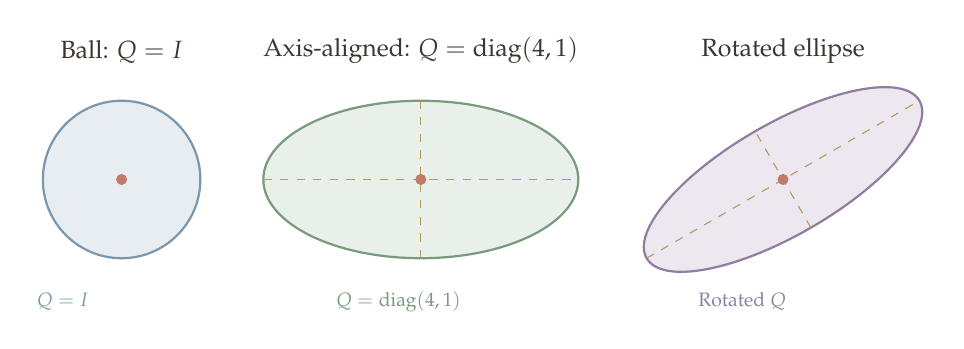
\begin{tikzpicture}

% Panel 1: Ball Q = I
\begin{scope}[shift={(0,0)}]
  % Fill and stroke the circle (radius 1)
  \fill[bluefill] (0,0) circle (1);
  \draw[stblue, thick] (0,0) circle (1);
  % Center dot
  \fill[terracotta] (0,0) circle (2pt);
  % Label
  \node[above, dkbrown, font=\small] at (0,1.35) {Ball: $Q = I$};
  % Legend
  \node[stblue, font=\scriptsize, right] at (-1.2,-1.55) {$Q = I$};
\end{scope}

% Panel 2: Axis-aligned Q = diag(4,1)
\begin{scope}[shift={(3.8,0)}]
  % Ellipse: semi-axes 2, 1
  \fill[sagefill] (0,0) ellipse (2 and 1);
  \draw[sage, thick] (0,0) ellipse (2 and 1);
  % Principal axes (dashed)
  \draw[rwgold, dashed, thin] (-2,0) -- (2,0);
  \draw[rwgold, dashed, thin] (0,-1) -- (0,1);
  % Center dot
  \fill[terracotta] (0,0) circle (2pt);
  % Label
  \node[above, dkbrown, font=\small] at (0,1.35) {Axis-aligned: $Q = \mathrm{diag}(4,1)$};
  % Legend
  \node[sage, font=\scriptsize, right] at (-1.2,-1.55) {$Q = \mathrm{diag}(4,1)$};
\end{scope}

% Panel 3: Rotated ellipse
% From Plotly: L = [[1.76776695, 0], [0.85732141, 0.8]]
% So Q = L L^T. Semi-axes along eigenvectors.
% Principal axis 1: (1.73205081, 1.0), length ~ 2
% Principal axis 2: (-0.35355339, 0.61237244), length ~ 0.707
\begin{scope}[shift={(8.4,0)}]
  % The ellipse is parameterized by x = 1.76776695 cos(t), y = 0.85732141 cos(t) + 0.8 sin(t)
  % We draw it using a rotated ellipse.
  % Eigenvalues of Q = LL^T: compute angle
  % v1 direction: atan2(1.0, 1.73205081) = 30 degrees
  % Semi-axis lengths: |v1| = sqrt(1.73205081^2 + 1^2) = 2, |v2| = sqrt(0.35355339^2 + 0.61237244^2) = 0.7071
  \begin{scope}[rotate=30]
    \fill[lavfill] (0,0) ellipse (2 and 0.7071);
    \draw[lavender, thick] (0,0) ellipse (2 and 0.7071);
  \end{scope}
  % Principal axes (in original coords)
  \draw[rwgold, dashed, thin] (-1.73205081,-1.0) -- (1.73205081,1.0);
  \draw[rwgold, dashed, thin] (0.35355339,-0.61237244) -- (-0.35355339,0.61237244);
  % Center dot
  \fill[terracotta] (0,0) circle (2pt);
  % Label
  \node[above, dkbrown, font=\small] at (0,1.35) {Rotated ellipse};
  % Legend
  \node[lavender, font=\scriptsize, right] at (-1.2,-1.55) {Rotated $Q$};
\end{scope}

\end{tikzpicture}
\end{document}
